\section{Temporal Verification} \label{sec:temp}
In the temporal verification stage, we will use the path information that we got from 
functional verification stage and augment them with latency information to 
produce the final temporal property probability.

\begin{figure}[h]
    \centering
    % 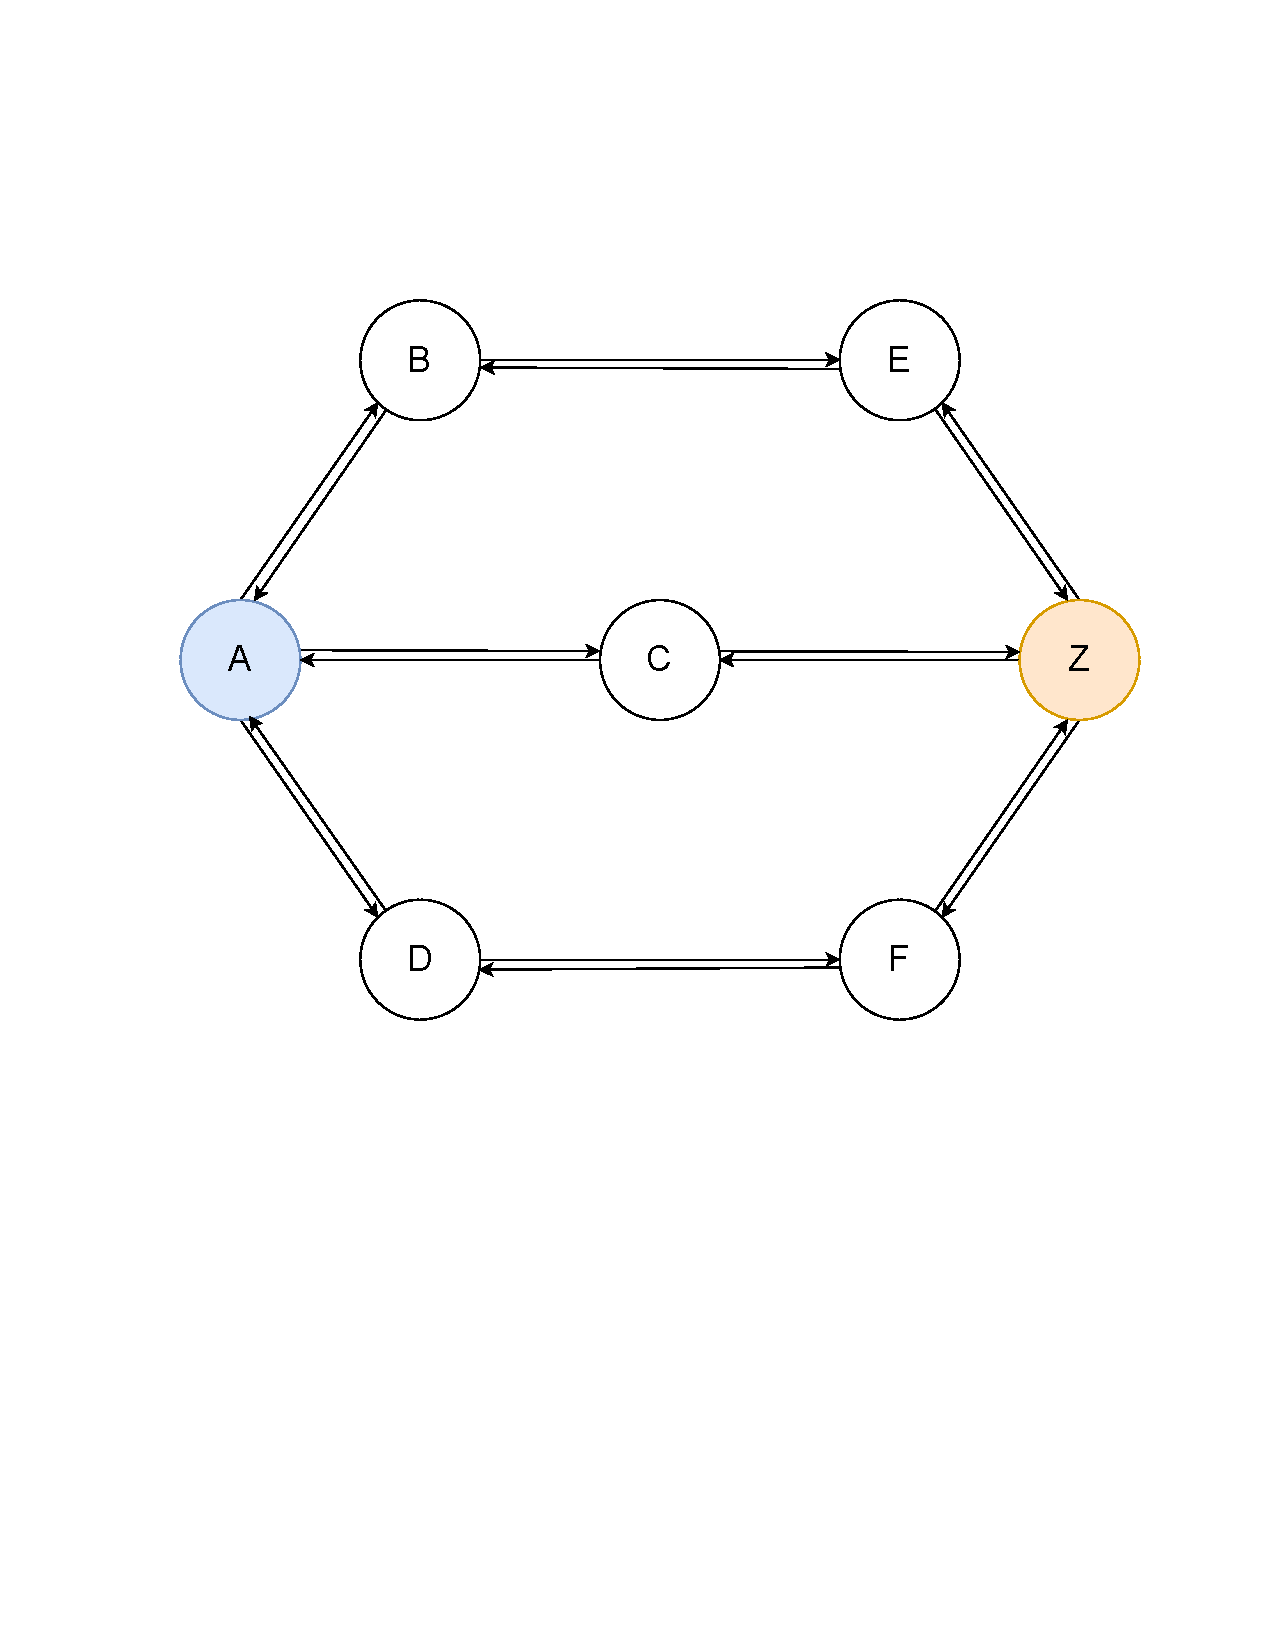
\includegraphics[width=0.4\textwidth, trim=0cm 11cm 0cm 5cm]{ex.pdf}
    \includegraphics[width=\columnwidth]{../tikz/tree}
    % 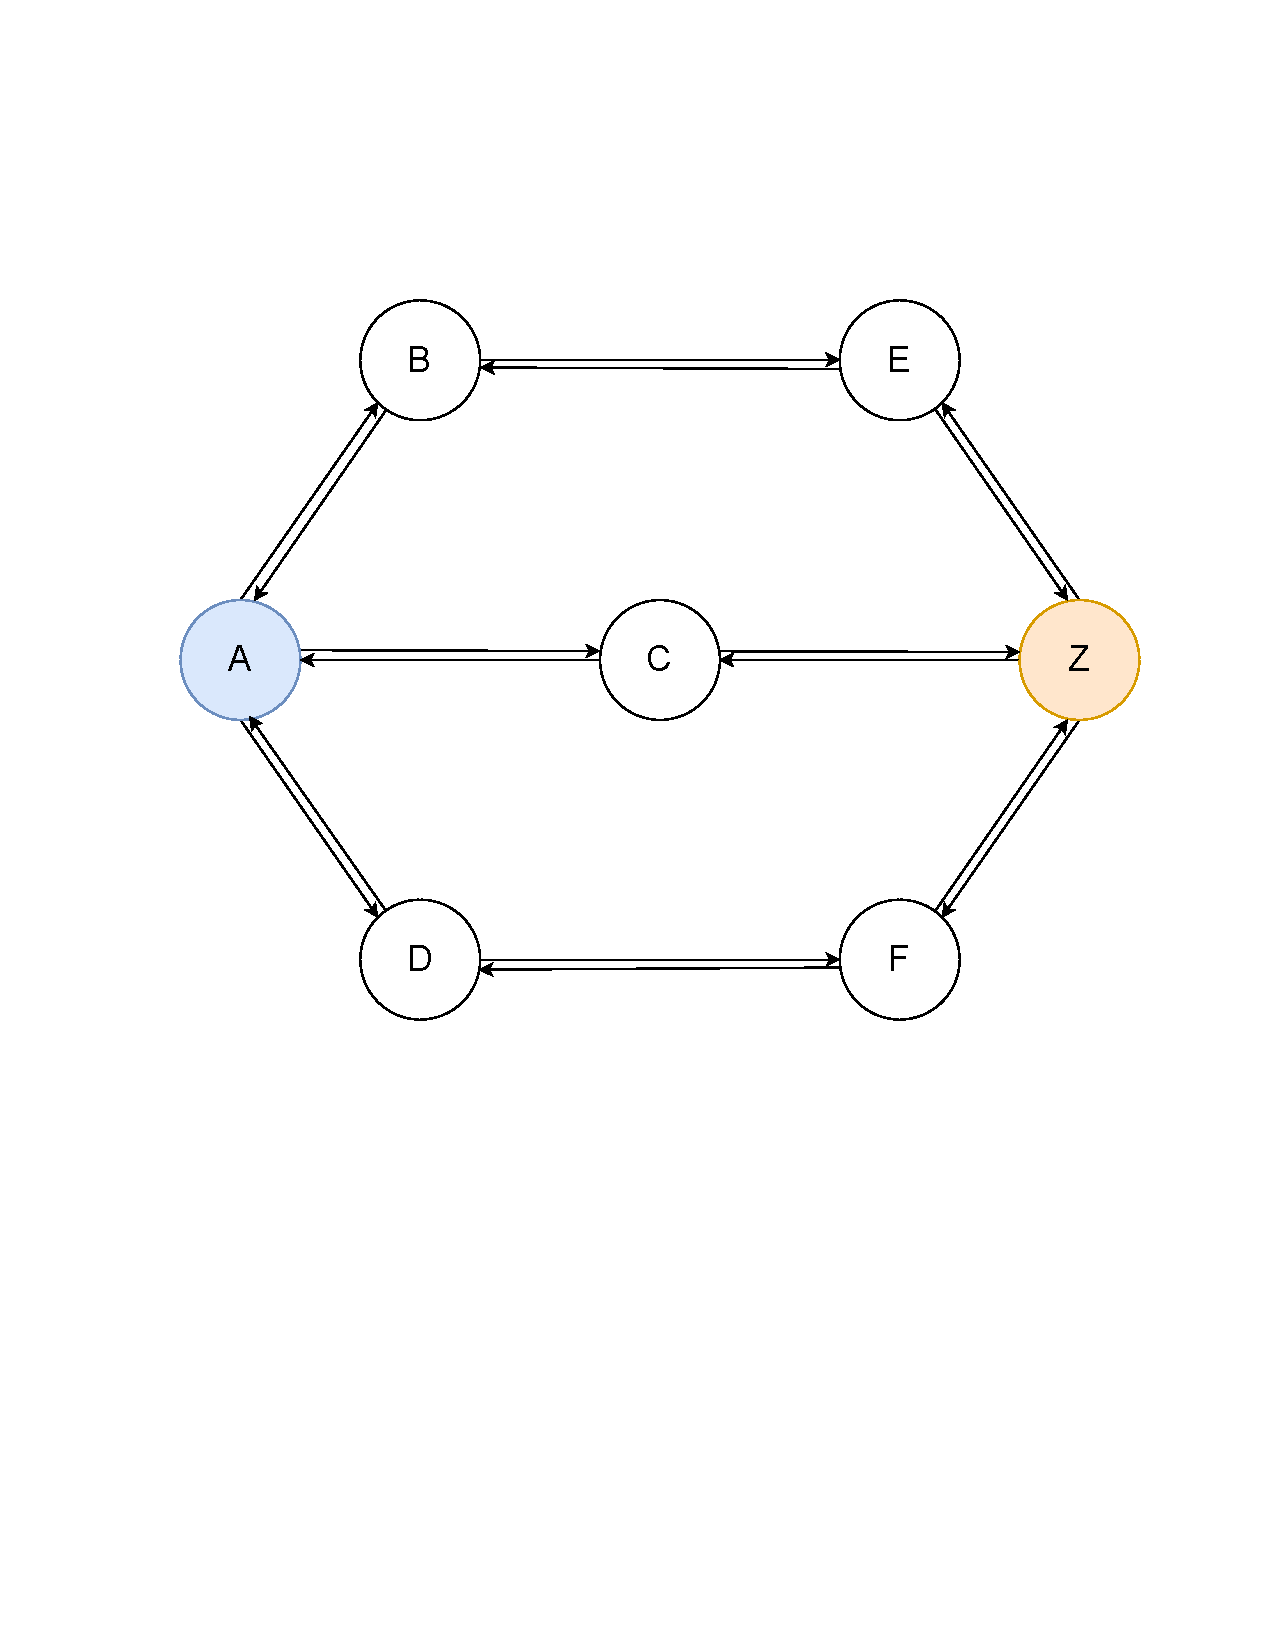
\includegraphics{ex.eps}
    \caption{Subset of Modified Exploration Tree $\mathcal{T}$ for our example topology, 
        $\mathcal{E}_2$ and $\mathcal{E}_3$ will get consolidated}
    \label{fig:tree}
\end{figure}

\subsection{Latency Label}
Similar to link failure $r$, we use edge-labeling technique to represent latency that 
will get introduced by the connectivity between two nodes. 
Our model will model two significant sources of latency: \textbf{link propagation} 
and \textbf{packet queuing in the node}.
We will encode these latencies by equipping the model with two additional labels.

Encoding link propagation latency is fairly straightforward. 
We define a function $l_p: E_t \rightarrow \mathcal{D}$ where $\mathcal{D}$ is a set of 
continuous univariate distribution that has a minimum value of $0$.
This distribution signifies the time it would take for the respective physical link to transmit 
a packet from one end to another.
Because of this, just like $r$, two symmetrical edges will share the same distribution.

To encode queuing latency, we first note that the queuing mechanism in modern switches 
usually resides in the output port. %TODO: Cite PISA?
Since a port in a switch is only connected to one other port, we could effectively 
assign the latency to the connectivity between switches.
To do this, we define another function $l_q: E_t \rightarrow \mathcal{D}$.
This distribution signifies the output queue latency in the source node that is 
going to be forwarded to the destination node.
Unlike $l_p$, two symmetrical edges will have two different distributions since they 
represent two different output queues.

In our running example, we will assume that all edges in the topology will have $l_p$
and $l_q$ of gamma distribution with $\lambda = 1$, except $l_q(EZ)$ which will 
have a lognormal distribution with $\alpha = 1$ and $\theta = 1$.

Given $paths$, $l_p$, and $l_q$, we could then compute $P_t$, the probability of a 
given temporal property being fulfilled.
We will describe our algorithm for computing this probability in the next few 
sections.

\subsection{Weighted Average and Path Convolution}
Since a convergent behavior of the forwarding plane $paths$ might contain more than 
one paths, we will compute the temporal probability of $paths$ by computing the 
weighted average of the temporal probability of each of the individual path.
The specific weight depends on the load-balancing method used.
%We have implemented the weight computation for ECMP load-balancing scheme.

To get the temporal probability of a single path, we will use the latency information 
from $l_p$ and $l_q$ to compute the latency distribution of the whole path.
To do this, we resort to the methods of \textbf{convolution}.
For each edge $e$ in the path, we will get $l_p(e)$ and $l_q(e)$ and convolve them 
all together to get the path latency distribution.

With this path latency distribution, we could get the temporal probability of a 
path by computing the statistical property of said distribution.
In this work, given a path latency distribution $\mathcal{L}$, we define two temporal 
properties:
\begin{itemize}
    \item \textbf{Bounded Reachability}: the probability that a packet will get 
        transmited below $t$ time unit. This will get computed as $cdf(\mathcal{L}, t)$
    \item \textbf{Tail Reachability}: the probability that a packet will get 
        transmited above $t$ time unit. This will get computed as 
        $1 - cdf(\mathcal{L}, t)$
\end{itemize}

In our Fig. \ref{fig:tree} Exploration Tree for example, $\mathcal{E}_2$ has two 
equally probable path, $ABEZ$ and $ADFZ$.
We will first do a chain convolution of all the distributions in $ABEZ$ ($l_p(AB)$, 
$l_q(AB)$, ..., $l_q(EZ)$) and do the same thing for $ADFZ$.
We will then take the $CDF$ of $\mathcal{L}_{ABEZ}$ and $\mathcal{L}_{ADFZ}$ with our 
desired $t$ and average them out to get $P_t$ of $\mathcal{E}_2$. 

In short, given $paths$, $l_p$, and $l_q$, we will do the following:
\begin{enumerate}
    \item Split $paths$ into its individual path
    \item For each path, compute its latency distribution by convolving the latency distribution 
        $l_p$ and $l_q$ of each link
    \item With the resulting path latency distribution, determine the probability of temporal 
        property by computing the statistical property of said distribution
    \item Combine the temporal property of each path by computing the weighted average, based 
        on the load-balancing scheme of the control plane
\end{enumerate}

We do each of these steps to every Equivalence Class in $\mathcal{T}$, and do a sum-product operation 
of $P_f$ and $P_t$ to get the final probability of the property in question.

By introducing the temporal verification algorithm, we're essentially adding additional overhead to the 
exploration algorithm (on top of functional verification) that scales to the size of the Exploration Tree.
In other words, for $\mathcal{T}$ of size $n$, we will need to do temporal verification in each of 
those $n$ Equivalence Class.
We aim to minimize the overhead of temporal verification by introducing some optimization algorithms
later.

\subsection{Numeric Convolution}
However, there is one major problem with a convolution-based technique for computing the latency distribution 
of a given path: not every distribution pair can be convolved analytically.
A closed-form solution of a convolution is usually only available for two distributions of the same type.

In our example, we define $l_q(EZ)$ to be lognormal distribution, which doesn't have a closed form convolution 
solution with the other latency distribution in the network, which is of gamma distribution form.
Therefore, in order to convolve two arbitrary distributions, we need to leverage a numerical convolution 
method.

We leverage an existing numerical convolution algorithm, DIRECT, to fulfill this role.
%TODO: describe DIRECT in one sentence
We choose this method due to their bounded error property: DIRECT guarantee that the computed 
distribution and the correct theoretical distribution has a KL-divergence below a certain bound.
DIRECT has also been implemented in R's popular bayesmeta package.
%TODO: cite and change font?

One subtle detail about DIRECT is while convolution is defined to be a commutative operation, and 
DIRECT also achieves this property, the order of operation matters for the algorithm's runtime 
performance.
In particular, if we had a chain of DIRECT convolutions, the result of a convolution should not be set 
as the second input distribution in the later convolutions to avoid performance penalty.
This is caused by a nested loop from the following two mechanisms:
\begin{itemize}
    \item DIRECT works by computing a list of support values by doing many PDF queries of the second input
        distribution
    \item Computing the PDF of a DIRECT distribution (the returned distribution of a DIRECT 
        algorithm) itself involves iterating over the current support values
\end{itemize}

As an ilustration, if we had 3 random variables $A$, $B$, and  $C$, and we want 
to convolve them all together, it would be faster to compute $direct(direct(A, B), C)$ instead of 
$direct(C, direct(A, B))$.

While this problem is trivial to solve (swap the input parameter if the latter is detected as a 
DIRECT distribution), it does limit the type of optimization that we could have in the chain convolution 
process.
